% /* GRASP: Copyright 1997,1998  Bruce Allen */
% $Id: man_40meter.tex,v 1.24 1999/11/22 15:48:22 ballen Exp $
\section{GRASP Routines: Reading/using Caltech 40-meter prototype data}
\setcounter{equation}0
\label{s:40meter}
{\bf
This Section of the GRASP manual is now OBSOLETE
(except for historical interest)  - it describes the OLD
1994 40-meter data format.  The 40-meter data from 1994 has been
translated into FRAME format, and is distributed in FRAME format only.
Please go to Section~\ref{s:frameformat} of the GRASP manual, which contains details about the FRAME format 1994 data.
}

There is a good archive of data from the Caltech 40-meter prototype
interferometer.
(Note that this name is slightly misleading: the average length of the optical
arm cavities is 38.25 meters.)
Although the interferometer is only sensitive enough
to detect events like binary inspiral within $\approx$ 10kpc (the
distance to the galactic center) its output is nevertheless very useful
in studying data analysis algorithms on real-world interferometer
noise.  This data was taken during the period from 1993 to 1996; for
our purposes here we will concentrate on data taken during a one-week
long observation run from November 14-21, 1994.  The original data is
contained on 11 exabyte tapes with about 46 total hours of data; the
instrument was in lock about 88\% of the time.  The details of this
run, the status of the instrument, and the properties of this data are
well-described in theses by Gillespe \cite{Gillespie} and Lyons
\cite{Lyons}.

The GRASP package includes routines for reading this data.  The data is
not read directly from the tapes themselves; the data instead must be
read off the tapes and put onto disk (or into pipes) using a program
called {\tt extract}.  The GRASP routines can then be used to read
the resulting files.  While the GRASP routines can be used without any
further understanding of the data format, it is very helpful to understand
this in more detail.  Note that these data formats and the associated
structures were defined years before GRASP was written; we did not choose
this data format and should not be held accountable for its shortcomings.
We have included a preliminary translator that translates the data from
this old 1994 format into the new LIGO/VIRGO frame format.  The program
{\tt translate} may be found in the GRASP {\tt src/examples/examples\_utility} directory,
and is documented in the Section on GRASP general purpose utilities.

If you want to develop or work on data analysis algorithms, you will
want to have access to this data archive.  Because many people
contributed to taking this data, and because the LIGO project wants to
maintain control of its use and distribution, {\it this data set is NOT
in the public domain}.  However, you may request a copy for your use,
or for use by your research group.  Write to: Director of the LIGO
Laboratory, Mail Stop 51-33, California Institute of Technology,
Pasadena, CA 91125.  The data set is available in {\tt tar} format on
two Exabyte 8500c format tapes.  Each directory (for a different run
on a different day) occupies the following amount of space (in mbytes):
{\tt
\begin{verbatim}
             14nov94.1    647
             14nov94.2    913
             18nov94.1   1041
             18nov94.2   1121
             19nov94.1   1554
             19nov94.2   1074
             19nov94.3   1250
             19nov94.4   1206
             20nov94.1   1146
             20nov94.2   1173
             20nov94.3   1543
\end{verbatim}
}
\noindent
Each of these directories contains the {\tt channel.*} files and the {\tt
swept-sine.ascii} swept-sine calibration files.  In this manual, we assume
that these directories (or links to them) have been placed where you can
access them.  The GRASP programs that use this data determine its location
by means of the environment variable {\tt GRASP\_DATAPATH}.  You can
set this by typing (for example)\\ \indent {\tt setenv GRASP\_DATAPATH
/usr/local/data/19nov94.3}\\ to access the data from run 3 on November
19th.  System administrators: after installing these directories in a
convenient place on your machine, we recommend that you install a set of
links to them in the directory {\tt data} within the GRASP home directory.
This way your users can find them without asking you for the location!

WARNING:  this data was written on a ``big-endian" machine (the sun-4
workstation is an example of such a machine).  The floats are in IEEE
754 floating-point format.  Attempts to read the data in its
distributed form on a ``little-endian" machine (such as Intel 80*86
computers) will yield garbage unless the bytes are properly swapped.
The routines used to read data (in particular, the function {\tt
read\_block()}) test the byte order of the machine being used, and swaps
the byte order if the machine is ``little-endian".  This introduces
some inefficiency if you are running on a ``little-endian" machine, but
is preferrable to having two copies of the data, one for each
architecture.  If you are doing all of your work on a ``little-endian"
machine and you want to avoid this inefficiency, write a program which
properly swaps the byte orders of the header blocks (which are in
4-byte units) and then also properly swaps the byte order of the data
blocks (which are 2-byte units) and reformat the raw data files.  Then
modify the {\tt read\_block()} data so that it no longer swaps the bytes
on your machine.

\subsection{The data format}
\setcounter{equation}0
Data is written onto the exabyte tapes in blocks about 1/2 megabyte in
size.  The format of the data on the tapes is as shown in
Table~\ref{t:datatape}.
\begin{table}[h]
\begin{tabular}[]{|c|c|c|c|c|c|c|c|c|c|c|c|c|c|c}
\hline
mh & 0's & 0's & mh & 0's & 0's &  mh &gh & 0's & data & mh &gh & 0's & data & $\cdots$ \\
\hline
\multicolumn{2}{|c|}{1024} & 1024 &  \multicolumn{2}{|c|}{1024}  & 1024 & \multicolumn{3}{|c|}{1024} &  $1024 \times n$ & 
 \multicolumn{3}{|c|}{1024} &  $1024 \times n$& $\cdots$\\
\hline
\end{tabular}
\caption{Format of Exabyte data tapes (first row: content, second row: length in bytes).}
\label{t:datatape}
\end{table}
The tape begins with a main header (denoted ``mh" in the table).  This
is followed by a set of zeros, padding the length of the header block
to 1024 bytes.  There is then an empty block of 1024 bytes containing
zeros.  This pattern is repeated until the first block containing
actual data.  This is signaled by the appearance of a main header,
followed by a gravity header (denoted ``gh" in the figure above).
These two headers are padded with zeros to a length of 1024 bytes.
This is then followed by a set of data (the length of this set is a
multiple of 1024 bytes).  Information about the length of the data sets
is contained in the headers.  The data sets themselves consist of data
from a total of 16 channels, each of which comes from a 12-bit A to D
converter.  Four of the 16 channels are fast (sample rates a bit slower
than 10kHz) and the remaining 12 channels are slow (sample rates a bit
slower than 1kHz).  The ratio of sample rates is exactly $10:1$.
Within the blocks labeled ``data", these samples are interleaved.  The
information content of the different channels is detailed on page 136
of Lyon's thesis \cite{Lyons}, and is summarized in Table~\ref{t:chassign}.

The program {\tt extract} reads data off the tapes and writes them into
files.  One file is produced for each channel; typically these files
are named {\tt channel.0} $\rightarrow$ {\tt channel.15}.  The complete
set of these files for the November 1994 run fits onto two Exabyte
tapes (in the 8500c compressed format).  The information in these files
begins only at the moment when the useful data (starting with the
gravity header blocks) begins to arrive.  The format of the data in
these {\tt channel.*} files is shown in Table~\ref{t:datafile}.
\begin{table}[h]
\begin{tabular}[]{|c|c|c|c|c|c|c|c|c|c|c|c|c|c|c|c|c}
\hline
\multicolumn{4}{|c|}{block 0} &  \multicolumn{4}{|c|}{block 1} & \multicolumn{4}{|c|}{block 2}  &\multicolumn{4}{|c|}{block 3} & $\cdots$ \\
\hline
mh &bh & 0's               & data &mh &bh & 0's               & data & mh &bh & 0's              & data & mh &bh & 0's              & data & $\cdots$ \\ 
\hline
\multicolumn{3}{|c|}{1024} & cs   &\multicolumn{3}{|c|}{1024} & cs   &\multicolumn{3}{|c|}{1024} & cs   &\multicolumn{3}{|c|}{1024} & cs   & $\cdots$ \\ 
\hline
\end{tabular}
\caption{Format of a {\tt channel.0$\rightarrow$15} file (first row:
block number, second row: content, third row: length in bytes).}
\label{t:datafile}
\end{table}
Here the main headers are the same as before, however the headers that
follow them are called binary headers (denoted by ``bh" in the table).
The length of the data stream (in bytes) is called the ``chunksize" and
is denoted by ``cs" in Table~\ref{t:datafile}.  We frequently reference
the data in these files by ``block number" and ``offset".  The block
number is an integer $\ge 0$ and is shown in Table~\ref{t:datafile}.
The offset is an integer which, within a given block, defines the
offset of a data element from the first data element in the block.  In
a block containing 5000 samples, these offsets would be numbered from 0
to 4999.

The structure of the binary headers is\\
{\tt struct ld\_binheader \{}
\begin{description}
  \item{\tt float elapsed\_time:} This is the total elapsed time in
  seconds, typically starting from the first valid block of
    data, from the beginning of the run.
  \item{\tt float datarate:}  This is the sample rate of the channel, in Hz.
\end{description}
\};

The structure of the main headers is\\
{\tt struct ld\_mainheader \{}
\begin{description}
  \item{\tt  int chunksize:} The size of the data segment that follows, in bytes.
  \item{\tt  int filetype:} Undocumented; often 1 or 2.
  \item{\tt  int epoch\_time\_sec:} The number of seconds after January 1, 1970, Coordinated
   Universal Time (UTC) for the first sample.  This is the quantity returned by the function {\tt time()} in the
   standard C library.  
  \item{\tt  int epoch\_time\_msec:} The number of millseconds which should be added to the previous quantity.
  \item{\tt  int tod\_second:} Seconds after minute, 0-61 for leap second, local California time.
  \item{\tt  int tod\_minute:} Minutes after hour 0-59, local California time.
  \item{\tt  int tod\_hour:} Hour since midnight 0-23, local California time.
  \item{\tt  int date\_day:} Day of the month, 1-31, local California time.
  \item{\tt  int date\_month:} Month of the year, 0-11 is January-December, local California time.
  \item{\tt  int date\_year:} Years since 1900, local California time.
  \item{\tt  int date\_dow:} Days since Sunday, 0-6, local California time.
  \item{\tt  int sub\_hdr\_flag:} Undocumented.
\end{description}
\};
Note: in the original headers, these {\tt int} were declared as {\tt
long}.  They are in fact 4-byte objects, and on some modern machines,
if they are declared as long they will be incorrectly interpreted as
8-byte objects.  For this reason, we have changed the header definitions
to what is show above.  Also please note that the time values ${\tt tod\_minute}
\cdots {\tt date\_year}$ are the local California time, not UTC.

For several years, the {\tt extract} program contained several bugs.
One of these caused the {\tt channel.*} to have no valid header
information apart from the {\tt elapsed time} and {\tt datarate}
entries in the binary header, and the {\tt chunksize} entry in the main
header.  All the remaining entries in the main header were either
incorrect or nonsensical.  This bug was corrected by Allen on 14
November 1996; data files produced from the tapes after that time should
have valid header information.

There was also a more serious bug in the original versions of {\tt
extract}.  The typical chunksize of most slow channels is 10,000 bytes
(5,000 samples) and the chunksize of most fast channels is 100,000
bytes (50,000 samples) but until it was corrected by Allen on 14
November 1996, the {\tt extract} program would in apparently
unpredictable (though actually quite deterministic) fashion  ``skip"
the last data point from the slow channels or the last ten data points
from the fast channels, giving rise to sequences of 4,999 samples from
the slow channels, and correspondingly 49,990 samples from the fast
channels.  Not surprisingly, these missing data points gave rise to
strange ``gremlins" in the early data analysis work; these are
described in Lyon's thesis \cite{Lyons} on pages 150-151.  These
missing points were simply cut out of the data stream as shown in
Figure~\ref{f:dropout}; rather like cutting out 1 millisecond of a
symphony orchestra every 5.1 seconds; this gives rise to ``clicks"
which excited the optimal filters.  This problem is shown below; data
taken off the tapes after 14 November 1996 should be free of these
problems.

There are a couple of caveats regarding use of these ``raw data" files.
First, in the {\tt channel.*} files, there can be, with no warning,
large segments of missing data.  In other words, a block of data with
time stamp 13,000 sec, lasting 5 sec, can be followed by another data
block with a time stamp of 14,000 sec (i.e., 995 sec of missing data).
Also, the time stamps are stored in single precision floats, so that
after about 10,000 sec they no longer have a resolution better than a
single sample interval.  When we read the data, we typically use the
time-stamp on the first data segment to establish the time at which the
first sample was taken. Starting from that time, we then determine the
time of a data segment by using {\tt elapsed\_time}, since the millisecond
time resolution of {\tt epoch\_time\_msec} is not good enough.  (See the
comments in Section~\ref{ss:timestamp}).

For our purposes, the most useful channels are {\tt channel.0} and {\tt
channel.10}.  Channel 0 contains the actual voltage output of the IFO.
This is typically in the range of $\pm 100$.  Later, we will discuss
how to calibrate this signal.  Channel 10 contains a TTL locked level
signal, indicating if the interferometer was in lock.  This is typically
in the range from 1 to 10 when locked, and exceeds several hundred when
the interferometer is out of lock.  Note: after coming into lock you
will notice that the IFO output is often zero (with a bit of DC offset)
for periods ranging from a few seconds to a minute.  This is because
the instrument output amplifiers are typically overloaded (saturated)
when the instrument is out-of-lock.  Because they are AC coupled,
this leads to zero output.  After the instrument comes into lock, the
charge on these amplifiers gradually bleeds off (or one of the operators
remembers to hit the reset button) and then the output ``comes alive".
So don't be puzzled if the instrument drops into lock and the output is
zero for 40 seconds afterwards!

\begin{figure}[hb]
\index{colorpage}
\begin{center}
\epsfig{file=Figures/figure10.ps,angle=270,width=5in}
\caption{ \label{f:dropout} This shows the appearance of {\tt
channel.0} before and after the {\tt extract} program was repaired (on
14 November 1996) to correctly extract data from the Exabyte data
tapes. The old version of {\tt extract} dropped the ten data points
directly above the words ``missing data"; in effect these were
interpolated by the diagonal line (but with ten times the slope shown
since everything in between was missing).}
\end{center}
\end{figure}

The contents of the {\tt channel.*} files was not the same for all of
the runs.  Lyon's thesis \cite{Lyons} gives a chart on page 136 with
some ``typical" channel assignments.  The channel assignments during
these November 1994 data runs are listed in a log book; they were
initially chosen on November 14, then changed on November 15th and
again on November 18th; these assignments are shown in
Table~\ref{t:chassign}.   (Note that the chart on page 136 of Lyon's
thesis describes the channel assignments on 15 November 94, a day when
no data was taken.)

\begin{table}[h]
\begin{tabular}[]{c|c|c}
\hline
Channel Number &  Description $\le$ 14 November 94 & Description $\ge$ 18 November 94 \\
\hline
0 & IFO output & IFO output \\
1 & unused & magnetometer \\
2 & unused & microphone \\
3 & microphone & unused \\
\hline
4 & dc strain & dc strain \\
5 & mode cleaner pzt & mode cleaner pzt \\
6 & seismometer & seismometer \\
7 & unused & slow pzt\\
8 & unused&  power stabilizer \\
9 & unused  & unused  \\
10 & TTL locked &  TTL locked \\
11 & arm 1 visibility& arm 1 visibility \\
12 & arm 2 visibility &  arm 2 visibility\\
13 & mode cleaner visibility & mode cleaner visibility \\
14 & slow pzt &  unused \\
15 & arm 1 coil driver & arm 1 coil driver \\
\hline
\end{tabular}
\caption{Channel assignments for the November 1994 data runs.  Channels
0-3 are the ``fast" channels, sampled at about 10 kHz; the remaining
twelve are the ``slow" channels, sampled at about 1KHz.}
\label{t:chassign}
\end{table}
\clearpage
\subsection{Function: {\tt read\_block()}}
\setcounter{equation}0
{\tt int read\_block(FILE *fp,short **here,int *n,float *tstart,float *srate,int allocate,int *nalloc,int seek,
struct ld\_binheader* bh,struct ld\_mainheader* mh)}\\
This function efficiently reads one block of data from one of the {\tt
channel.*} data files, operating in sequential (not random) access.
On first entry, it detects the byte-ordering of the machine that it is
running on, and swaps the byte order if the machine is ``little-endian"
(the data was originally written in ``big-endian" format, and is
distributed that way).  It will also print a comment (on first entry)
if the machine is not big-endian.

The arguments are:
\begin{description}
\item{\tt fp:} Input.  A pointer to the {\tt channel.*} file being read.
\item{\tt here:} Input/Output. A pointer to an array of shorts, which
is where the data will be found when {\tt read\_block()} returns.  If
{\tt allocate}=0, then this pointer is input.  If {\tt allocate} is
non-zero, then this pointer is output.
\item{\tt n:} Output.  A pointer to an integer, which is the number of
data items read from the block, and written to {\tt *here}.  These data
items are typically short integers, so the number of bytes output is
twice *n.
\item{\tt tstart}: Output.  The time stamp (elapsed time since beginning of
the run) at the start of the data block.  Taken from the binary
header.
\item{\tt srate}: Output.  The sample rate, in Hz, taken from the binary
header.
\item{\tt allocate}:  Input.   The {\tt read\_block()} function  will place the
data that it has read in a user defined array if {\tt allocate} is
zero.  If {\tt allocate} is set, it will use {\tt malloc()} to allocate
a block of memory, and set {\tt *here} to point to that block of
memory.  Further calls to {\tt read\_block()} will then use calls to {\tt
realloc()} if necessary to re-allocate the size of the block of memory,
to accommodate additional data points.  Note that in either case, {\tt
read\_block()} puts into the array only the data from the next block; it
over-writes any existing data in memory.
\item{\tt nalloc}: Input/Output.   If {\tt allocate} is zero, then this is
used to tell {\tt read\_block()} the size (in shorts) of the array {\tt
*here}.  An error message will be generated by {\tt read\_block()} if
this array is too small to accommodate the data.  If {\tt allocate} is
nonzero, then this integer is set (and reset, if needed) to the number
of array entries allocated by {\tt malloc()/realloc()}.  In this case, be
sure that {\tt *nalloc} is zero before the first call to {\tt read\_block()},
or the function will think that it has already allocated memory!
\item{\tt seek:} Input.  If {\tt seek} is set to zero, then the function
reads data.  If {\tt seek} is set nonzero, then  {\tt read\_block()}
does not copy any data into {\tt *here}.  Instead it simply skips over
the actual data.
\item{\tt bh:} Output.  A pointer to the binary header structure defined above.
\item{\tt mh:} Output.  A pointer to the main header structure defined above.
\end{description}

This is a low-level function, which reads a block of data.  It is
designed to either write the data into a user-defined array or block of
memory, if {\tt allocate} is off, or to allocate the memory itself.  In
the latter mode, the function uses {\tt nalloc} to track the amount of
memory allocated, and reallocates if necessary. 
It is often useful to be able to quickly skip over sections of data
(for example, just after the interferometer locks, a few minutes
is needed for the violin modes to damp down).  Or if the IFO is out of
lock, one needs to quickly read ahead to the next locked section.
If {\tt seek} is set, then this routine behaves exactly as it would in
normal (read) mode but does not copy any data.

The function {\tt read\_block()} returns the number of data items that
will be returned on the {\it next} call to {\tt read\_block()}.  It
returns -1 if it has just read the final block of data (implying that
the next call will return 0).  It returns 0 if it can not read any
further data, because none remains.

Note that if the user has set {\tt allocate}, then the {\tt
read\_block()} will allocate memory using {\tt malloc()/realloc()}.  It
is the users responsibility to free this block of memory when it is no
longer needed, using {\tt free()}.

\begin{description}
\item{Author:}  Bruce Allen, ballen@dirac.phys.uwm.edu
\item{Comments:}  This function was designed for variable-length blocks.  It might
be possible to simplify it for fixed-length block sizes.
\end{description}
\clearpage

\subsection{Example: {\tt reader} program}
\setcounter{equation}0
This example uses the function {\tt read\_block()} described in the
previous section to read the first 20 blocks out of the file {\tt
channel.0}.  It prints the header information for each block of data,
and the 100th data item from each block, along with the time associated
with that data item.

The data is located with the utility function {\tt grasp\_open()},
which is documented in Section~\ref{ss:graspopen}.  In order for
this example program to work, you {\it must} set the environment
variable {\tt GRASP\_DATAPATH} to point to a directory containing
40-meter data.  You can do this with a command such as\\
\indent {\tt setenv GRASP\_DATAPATH /usr/local/data/19nov94.3}\\
to access the data from run 3 on November 19th.

\lgrindfile{Includes/reader.tex}
\clearpage

\subsection{Function: {\tt find\_locked()}}
\setcounter{equation}0
{\tt 
int find\_locked(FILE *fp,int *s\_offset,int *s\_block,int *e\_offset,
int *e\_block,float *tstart,float *tend,float *srate)
}\\
This mid-level function looks in a TTL-locked signal channel
(typically, {\tt channel.10}) and finds the regions of time when the
interferometer is locked.  The first time it is called, it returns
information identifying the start and end times of the first locked
region.  The second time it is called it returns the start and end
times of the second locked region, and so on.

The arguments are:
\begin{description}
\item{\tt fp}: Input.  A pointer to the
  file containing the TTL lock signal.  A typical file name might be ``{\tt channel.10}".
\item{\tt s\_offset}: Output. The offset (number of shorts) into the
  block where the IFO locks.  This ranges from 0 to n-1 where the number
  of data items in block {\tt s\_block} is n.  This offset points to
  the first locked point.
\item{\tt s\_block}: Output. The number of the data block where the
  IFO locks.  This ranges from 0 to n-1 where the total number of data
  blocks in the file is n.
\item{\tt e\_offset}: Output. The offset (number of shorts) into the
  block where the IFO loses locks.  This ranges from 0 to n-1 where the
  number of data items in the block {\tt e\_block}.  This offset points
  to the last locked point (not to the first unlocked point).
\item{\tt e\_block}: Output. The number of the data block where the
  IFO loses lock.  This ranges from {\tt s\_block} to n-1 where the
  total number of data blocks in the file is n.
\item{\tt tstart}: Output. The elapsed time in seconds, since the
  beginning of the run, of the data block in which the first locked
  point was found.  Note:  This is not the time of lock acquisition!
\item{\tt tend}: Output.
  The elapsed time in seconds, since the beginning of the run, of the
  data block in which the last locked point was found.  Note:  this is
  not the time at which lock was lost!
\item{\tt srate}: Output. The sample rate of the TTL-locked channel, in Hz.
\end{description}

This routine uses {\tt read\_block()} to examine successive sections of
the {\tt channel.10} data file.  It looks for continuous sequences of
data points where the value lies between limits (inclusive) {\tt
LOCKL=1} and {\tt LOCKH=10}.  It returns the start and end points of
each successive such sequence.  The upper and lower limits can be
changed in the code, if desired, however these values appear to be
reliable ones.

The integer returned by {\tt find\_locked()} is the actual number of
data points in the {\it fast} channels, during the locked period.  It
returns 0 if there are no remaining locked segments.

If there is a gap in the data stream, arising not because the
instrument went out of lock, but rather because the tape-writing
program was interrupted and then later restarted, {\tt find\_locked()}
will print out a warning message, but will otherwise treat this simply
as a loss of lock during the period of the missing data.

\begin{description}
\item{Author:}  Bruce Allen, ballen@dirac.phys.uwm.edu
\item{Comments:}  This function was designed for variable-length blocks.  It might
be possible to simplify it for fixed-length block sizes.
\end{description}
\clearpage

\subsection{Example: {\tt locklist} program}
\setcounter{equation}0
This example uses the function {\tt find\_locked} described in the
previous section to print out location information and times for all
the locked sections in the file {\tt channel.10}.  Note that this
example only prints out information for locked sections longer than 30
sec.

\lgrindfile{Includes/locklist.tex}
\clearpage

\subsection{Function: {\tt get\_data()}}
\label{subsec:get_data}
\setcounter{equation}0
{\tt 
int get\_data(FILE *fp,FILE *fplock,float *tstart,int npoint,short *location,int *rem,float *srate,int seek)
}\\
This high-level function is an easy way to get the IFO output (gravity
wave signal) during periods when the IFO is locked.  When called, it
returns the next locked data section of a user-specified length.  It
also specifies if the section of data is part of a continuous locked
stream, or the beginning of a new locked section.

The arguments are:
\begin{description}
\item{\tt fp:} Input. Pointer to a file (typically {\tt channel.0})
containing the channel 0 data.
\item{\tt fplock:} Input. Pointer to a file
(typically {\tt "channel.10"}) containing the TTL lock
signal.
\item{\tt tstart:} Output.  The time of the zeroth point in the
returned data.
\item{\tt npoint:} Input.  The number of data points requested by the
user.
\item{\tt location:} Input.  Pointer to the location where the data
should be put.
\item{\tt rem:} Output.  The number of points of data remaining in this
locked segment of data.
\item{\tt srate:} Output.  The sample rate of the fast data channel, in Hz.
\item{\tt seek:} Input.  If this is zero, then the data is returned in
the array {\tt location[ ]}.  However if this input is non-zero, then
{\tt get\_data} performs exactly as described, except that it does not
actually read any data from the file or write to {\tt location[ ]}.
This is useful to quickly skip over un-interesting regions of the data,
for example the first several minutes after the interferometer acquires
lock.
\end{description}

This function returns 0 if there is no remaining locked data stream of
the requested length.  It returns 1 if it is just starting on a new
locked section of the data stream, and it returns 2 if the data is part
of an on-going locked sequence.

{\bf WARNING: } The {\tt get\_data()} function contains internal (static)
variables which mean that you can {\it not} use it as follows:
\begin{enumerate}
\item
Open a file pointer {\tt fp}
\item
Call {\tt get\_data(fp,$\cdots$)} some number of times
\item
Close the file pointer {\tt fp} and then (say) open it again
\item
Call {\tt get\_data(fp,$\cdots$)} some number of times.
\end{enumerate}
This sequence will leave you and the code very confused: it does not
correspond to ``rewinding" the file.  If this is desired then you
will have to modify the {\tt get\_data()} function by adding a helper
``reset()" function.

\begin{description}
\item{Author:}  Bruce Allen, ballen@dirac.phys.uwm.edu
\item{Comments:}  This function was designed for variable-length blocks.
It is possible to simplify it for fixed-length block sizes.  It should
also be modified to return a complete set of different channels, by
adding additional arguments to specify which channels are desired and
where the data should be placed.  This could also be used to eliminate
the {\tt seek} argument.
\end{description}
\clearpage

\subsection{Example: {\tt gwoutput} program}
\setcounter{equation}0
This example uses the function {\tt get\_data()} described in the
previous section to print out a two-column file containing the IFO
output for the first locked section containing 100 sample points.  In
the output, the left column is time values, and the right column is the
actual IFO output (note that because this comes from a 12 bit A-D
converter, the output is an integer value from -2047 to 2048).  The
program works by acquiring data 100 points at a time, then printing out
the values, then acquiring 100 more points, and so on.  Whenever a new
locked section begins, the program prints a banner message to alert the
user.  Note that typical locked sections contain $\approx 10^7$
points of data, so this program should not be used for real work --
it's just a demonstration!
\lgrindfile{Includes/gwoutput.tex}
\clearpage

\subsection{Example: {\tt animate} program}
\label{s:animate}
\setcounter{equation}0
This example uses the function {\tt get\_data()} described in the previous
section to produce an animated display showing the time series output
of the IFO in a lower window, and a simultaneously calculated FFT power
spectrum in the upper window.  This output from this program must be
piped into a public domain graphing program called {\tt xmgr}.  This may
be obtained from
\htmladdnormallink{{\tt http://plasma-gate.weizmann.ac.il/Xmgr/}.}
{http://plasma-gate.weizmann.ac.il/Xmgr/}
(This lists mirror sites in the USA and Europe also).
Some sample output of {\tt animate} is shown in Figure~\ref{f:animate}.
\begin{figure}[h]
\index{colorpage}
\begin{center}
\epsfig{file=Figures/figure7.ps,height=12cm,bbllx=15pt,bblly=60pt,
bburx=580pt,bbury=750pt}
\caption{ \label{f:animate} Snapshot of output from {\tt animate}.
This shows the (whitened) CIT 40-meter IFO a few seconds after acquiring
lock, before the violin modes have damped down }
\end{center}
\end{figure}

After compilation, to run the program type:\\
\indent {\tt animate $|$ xmgr -pipe \&} \\
to get an animated display showing the data flowing by and the power
spectrum changing, starting from the first locked data.  You can also
use this program with command-line arguments, for example\\ \indent
{\tt  animate 100 4 500 7 900 1.5 $|$ xmgr -pipe \&}\\ will show the
data from time $t= 100$ to time $t=104 $ seconds, then from $t=500$ to
$t=507$, then from $t=900$ to $t=901.5$.  Notice that the sequence of
start times must be increasing.

Note:  The {\tt xmgr} program as commonly distributed has a simple
bug that needs to be repaired, in order for the frequency scale of the
Fourier transform to be correct.  The corrected version of {\tt xmgr}
is shown in Figure~\ref{f:xmgrbug}.
\begin{figure}
\hrulefill
{\tt
\begin{verbatim}
        case 0:
==>        delt=(x[ilen-1]-x[0])/(ilen-1.0);
==>        T=(x[ilen-1]-x[0]);
           setlength(cg,specset,ilen/2);
           xx=getx(cg,specset);
...

        case 1:
==>        delt=(x[ilen-1]-x[0])/(ilen-1.0);
==>        T=(x[ilen-1]-x[0]);
\end{verbatim}}
\caption{\label{f:xmgrbug} The corrections to a bug in the {\tt xmgr}
program are indicated by the arrows above.  This bug is in the routine
{\tt do\_fourier()} in the file {\tt computils.c}. This bug has been repaired
in {\tt xmgr} version 4.1 and greater.}
\hrulefill
\end{figure}

\lgrindfile{Includes/animate.tex}
\clearpage

\subsection{Function: {\tt read\_sweptsine()}}
\setcounter{equation}0
{\tt 
void read\_sweptsine(FILE *fpss,int *n,float **freq,float **real,float **imag)}\\
This is a low-level routine which reads in a 3-column ASCII file of
swept sine calibration data used to calibrate the IFO.

The arguments are:
\begin{description}
\item{\tt fpss:} Input.  Pointer to a file in which the swept sine data can be
  found.  The format of this data is described below.
\item{\tt n:} Output.  One greater than the number of entries (lines) in the swept sine calibration file.
This is because the {read\_sweptsine} returns, in addition to this data, one additional entry at
frequency $f=0$.
\item{\tt freq:} Output.  The array {\tt *freq[1..*n-1]} contains the frequency values from the
 swept sine calibration file.  The routine adds an additional entry at DC, {\tt *freq[0]=0}.
 Note: the routine allocates memory for the array.
\item{\tt real:} Output.  The array {\tt *real[1..*n-1]} contains the real part of the response function of the
IFO.  The routine adds {\tt *real[0]=0}.  Note: the routine allocates memory for the array.
\item{\tt imag:} Output.  The array {\tt *imag[1..*n-1]} contains the imaginary part of the response function of the
IFO.  The routine adds {\tt *imag[0]=0}.  Note: the routine allocates memory for the array.
\end{description}

The swept sine calibration files are 3-column ASCII files, of the form:
\begin{center}
$f_1$ $\qquad$ $r_1$ $\qquad$ $i_1$ \\
$f_2$ $\qquad$ $r_2$ $\qquad$ $i_2$ \\
$\cdots$\\
$f_m$ $\qquad$ $r_m$ $\qquad$ $i_m$
\end{center}
where the $f_j$ are frequencies, in Hz, and $r_j$ and $i_j$ are
dimensionless ratios of voltages.  There are typically $m=801$ lines in
these files.  Each line gives the ratio of the IFO output voltage to a
calibration coil driving voltage, at a different frequency.  The $r_j$
are the ``real part" of the response, i.e. the ratio of the IFO output
in phase with the coil driving voltage, to the coil driving voltage.
The $i_j$ are the ``imaginary part" of the response, $90$ degrees out
of phase with the coil driving voltage.  The sign of the phase (or
equivalently, the sign of the imaginary part of the response) is
determined by the following convention.  Suppose that the driving
voltage (in volts) is
\begin{equation}
\label{e:calibrate1}
V_{\rm coil} = 10 \cos( \omega t) = 10 \Re {\rm e}^{i \omega t}
\end{equation}
where $\omega= 2 \pi \times 60 \> {\rm radians/sec}$ is the angular frequency of
a 60 Hz signal.  Suppose the
response of the interferometer output to this is (again, in volts)
\begin{eqnarray}
\label{e:calibrate2}
V_{\rm IFO} &=& 6.93 \; \cos(\omega t) + 4\; \sin(\omega t)\cr
 &=& 6.93 \; \cos(\omega t) - 4\; \cos(\omega t + \pi/2) \cr
 &=& 8 \; \Re {\rm e}^{i (\omega t - \pi/6)}
\end{eqnarray}
This is shown in Figure~\ref{f:phase}. 
An electrical engineer would describe this
situation by saying that the phase of the response $V_{\rm IFO}$ is lagging the
phase of the driving signal $V_{\rm coil}$ by $30^\circ$.  The corresponding line
in the swept sine calibration file would read:
\begin{center}
$\cdots$\\
$60.000$ $\qquad$ $0.6930$ $\qquad$ $-0.40000$\\
$\cdots$
\end{center}
Hence, in this example, the real part is positive and the imaginary
part is negative.  We will denote this entry in the swept sine
calibration file by $S(60) = 0.8 \; {\rm e}^{ -i\pi/6} = 0.693 - 0.400
i$.  Because the interferometer output is real, there is also a value
implied at negative frequencies which is the complex conjugate of the
positive frequency value:  $S(-60) = S^*(60) = 0.8 \; {\rm e}^{
i\pi/6} = 0.693 + 0.400 i$.

Because the interferometer has no DC response, it is convenient for us
to add one additional point at frequency $f=0$ into the output data
arrays, with both the real and imaginary parts of the response set to
zero.  Hence the output arrays contain one element more than the number
of lines in the input files.  Note that both of these arrays are
arranged in order of increasing frequency; after adding our one
additional point they typically contain 802 points at frequencies from
0 Hz to 5001 Hz.

For the data runs of interest in this section (from
November 1994) typically a swept sine calibration curve was taken
immediately before each data tape was generated.

\begin{figure}[t]
\begin{center}
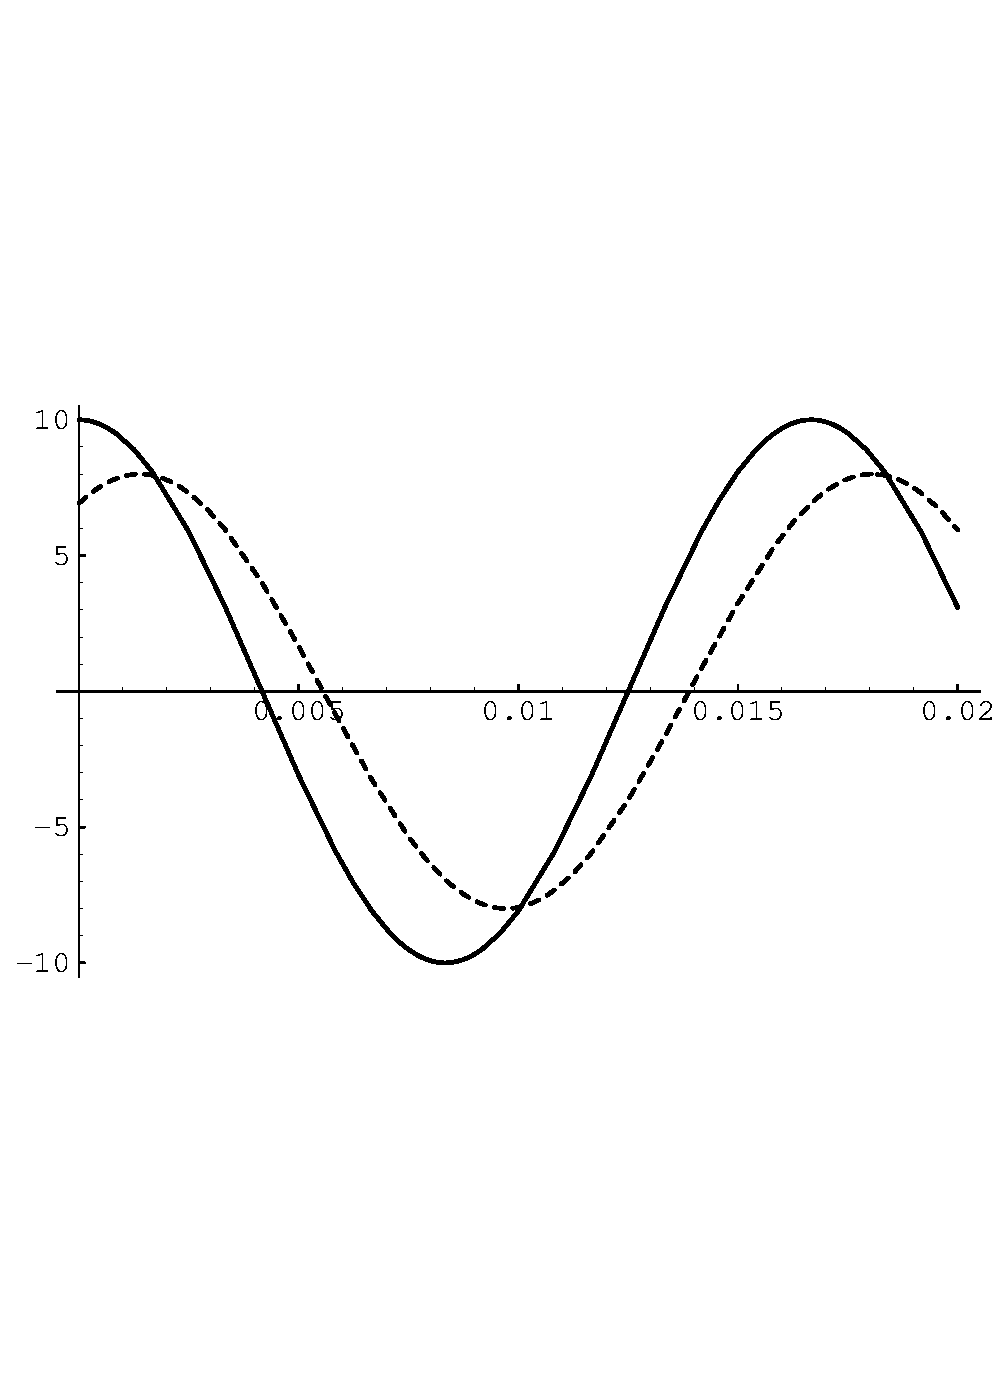
\epsfig{file=Figures/figure8.ps,height=5cm,bbllx=60pt,bblly=250pt,
bburx=550pt,bbury=530pt}
\caption{ \label{f:phase} This shows a driving voltage $V_{\rm coil}$
(solid curve) and the response voltage $V_{\rm IFO}$ (dotted curve) as
functions of time (in sec).  Both are 60 Hz sinusoids; the relative
amplitude and phase of the in-phase and out-of-phase components of
$V_{\rm IFO}$ are contained in the swept-sine calibration files.}
\end{center}
\end{figure}

We will shortly address the following question.  How does one use the
dimensionless data in the {\tt channel.0} files to reconstruct the
differential motion $\Delta l(t)$ (in meters) of the interferometer
arms?  Here we address the closely related question:  given $V_{\rm
IFO}$, how do we reconstruct $V_{\rm coil}$?  We choose the sign
convention for the Fourier transform which agrees with that of {\it
Numerical Recipes}:  equation (12.1.6) of \cite{NumRec}.  The Fourier
transform of a function of time $V(t)$ is
\begin{equation}
\label{e:fft1}
{\tilde V}(f) = \int {\rm e}^{2 \pi i f t} V(t) dt.
\end{equation}
The inverse Fourier transform is
\begin{equation}
\label{e:fft2}
V(t)= \int {\rm e}^{-2 \pi i f t} {\tilde V}(f) df.
\end{equation}
With these conventions, the signals (\ref{e:calibrate1}) and
(\ref{e:calibrate2}) shown in in Figure~\ref{f:phase} have Fourier
components:
\begin{eqnarray}
{\tilde V}_{\rm coil}(60) = 5                  \quad &{\rm and}& \quad {\tilde V}_{\rm coil}(-60) = 5,\\
{\tilde V}_{\rm IFO}(60)  = 4{\rm e}^{i \pi/6} \quad &{\rm and}& \quad {\tilde V}_{\rm IFO}(-60)  = 4 {\rm e}^{-i \pi/6}.
\end{eqnarray}
At frequency $f_0=60$ Hz the swept sine file
contains
\begin{equation}
S(60) = 0.8 \; {\rm e}^{-i \pi/6} \Rightarrow S(-60) = S^*(60) =
0.8 \; {\rm e}^{i \pi/6}.
\end{equation}
since $S(-f) = S^*(f)$.

With these choices for our conventions, one can see immediately from our
example (and generalize to all frequencies) that
\begin{equation}
\label{e:coilcon}
{\tilde V}_{\rm coil}(f) = {{\tilde V}_{\rm IFO} \over S^*(f)}.
\end{equation}
In other words, with the {\it Numerical Recipes} \cite{NumRec}
conventions for forward and reverse Fourier Transforms, the (FFT of
the) calibration-coil voltage is  the (FFT of the) IFO-output
voltage divided by the complex conjugate of the swept sine response.
\begin{description}
\item{Author:}  Bruce Allen, ballen@dirac.phys.uwm.edu
\item{Comments:}  The swept-sine calibration curves are usually quite
smooth but sometimes they contain a ``glitch" in the vicinity of
1 kHz; this may be due to drift of the unity-gain servo point.
\end{description}
\clearpage

\subsection{Function: {\tt calibrate()}}
\setcounter{equation}0
{\tt void calibrate(FILE *fpss,int num,float *complex,float srate,int
method,int order) }\\
This is a intermediate-level routine which reads in a 3-column ASCII
file of swept sine calibration data used to calibrate the IFO, and
outputs an array of interpolated points suitable for calibration of
FFT's of the interferometer output.

The arguments are:
\begin{description}
\item{\tt fpss:} Input.  Pointer to the file in which the
  swept sine data can be found.  The format of this data is described
  below.
\item{\tt srate:} Input.  The sample rate $F_{\rm sample}$ (in Hz) of the data that
  we are going to be calibrating.
\item{\tt num:} Input.  The number of points $N$ in the FFT that we
 will be calibrating.  This is typically $N=2^k$ where $k$ is an
 integer.  In this case, the number of distinct frequency values at
 which a calibration is needed is $2^{k-1}+1 = N/2+1$, corresponding to
 the number of distinct frequency values from $0$ (DC) to the Nyquist
 frequency $f_{\rm Nyquist}$.  See for example equation (12.1.5) of
 reference \cite{NumRec}.  The frequencies are $f_i = {i \over N}
 F_{\rm sample}$ for $i=0,\cdots,N/2$.
\item{\tt complex:} Input.  Pointer to an array {\tt complex[0..s]}
  where $s=2^k+1$.  The routine {\tt  calibrate()} fills in this array
  with interpolated values of the swept sine calibration data,
  described in the previous section.  The real part of the DC response
  is in {\tt complex[0]}, and the imaginary part is in {\tt
  complex[1]}. The real/imaginary parts of the response at frequency
  $f_1$ are in {\tt complex[2]} and {\tt complex[3]} and so on.  The
  last two elements of {\tt complex[ ]} contain the real/imaginary parts
  of the response at the Nyquist frequency $F_{\rm sample}/2$.
\item{\tt method:} Input.  This integer sets the type of interpolation
  used to determine the real and imaginary part of the response, at
  frequencies that lie in between those given in the swept sine
  calibration files.  Rational function interpolation is used if {\tt
  method}=0.  Polynomial interpolation is used if {\tt method}=1.
  Spline interpolation with natural boundary conditions (vanishing
  second derivatives at DC and the Nyquist frequency) is used if {\tt
  method}=2.
\item{\tt order:}  Input.  Ignored if spline interpolation is used.
  If polynomial interpolation is used, then {\tt order} is the order
  of the interpolating polynomial.
  If rational function interpolation is used, then the numerator and
  denominator are both polynomials of order {\tt order}/2 if {\tt order}
  is even; otherwise the degree of the denominator is ({\tt order}+1)/2
  and that of the numerator is ({\tt order}-1)/2.
\end{description}

The basic problem solved by this routine is that the swept sine
calibration files typically contain data at a few hundred distinct
frequency values.   However to properly calibrate the IFO output, one
usually needs this calibration information at a large number of
frequencies corresponding to the distinct frequencies associated with
the FFT of a data set.  This routine allows you to choose different
possible interpolation methods.  If in doubt, we recommend spline
interpolation as the first choice.  The interpolation methods are
described in detail in Chapter 3 of reference \cite{NumRec}.
\begin{description}
\item{Author:}  Bruce Allen, ballen@dirac.phys.uwm.edu
\item{Comments:}  It might be better to interpolate values of
$f^2$ times the swept-sine response function, as this is the quantity
needed to compute the IFO response function.
\end{description}
\clearpage

\subsection{Example: {\tt print\_ss} program}
\setcounter{equation}0
This example uses the function {\tt calibrate()} to read in a swept
sine calibration file, and then prints out a list of frequencies, real,
and imaginary parts interpolated from this data.  The frequencies are
appropriate for the FFT of a 4096 point data set with sample rate {\tt
srate}.   The technique used is spline interpolation.
\lgrindfile{Includes/print_ss.tex}

\clearpage
\subsection{Function: {\tt normalize\_gw()}}
\label{s:normalize}
\setcounter{equation}0
{\tt void normalize\_gw(FILE *fpss,int npoint,float srate,float *response)}

This routine generates an array of complex numbers $R(f)$ from the
information in the swept sine file and an overall calibration
constant.  Multiplying this array of complex numbers by (the FFT of)
{\tt channel.0} yields the (FFT of the) differential displacement of
the interferometer arms $\Delta l$, in meters: $\widetilde{\Delta l}(f)
= R(f) \widetilde{C_0}(f)$.  The units of $R(f)$ are meters/ADC-count.

The arguments are:
\begin{description}
\item{\tt fpss:} Input.  Pointer to the file in which the swept sine normalization
  data can be found.
\item{\tt npoint:} Input.  The number of points $N$ of {\tt channel.0} which will be used
to calculate an FFT for normalization.
Must be an integer power of 2.
\item{\tt srate:}  Input.  The sample rate in Hz of {\tt channel.0}.
\item{\tt response:} Output.  Pointer to an array {\tt response[0..s]}
with $s=N+1$ in which $R(f)$ will be returned.   By convention,
$R(0)=0$ so that {\tt response[0]=response[1]=0}.    Array elements
{\tt response[$2 i$]} and {\tt response[$2 i + 1$]} contain the real and
imaginary parts of $R(f)$ at frequency $f= i{\tt srate}/N$.   The
response at the Nyquist frequency {\tt response[N]=0} and {\tt
response[N+1]=0} by convention.
\end{description}

The absolute normalization of the interferometer can be obtained from
the information in the swept sine file, and one other normalization
constant which we denote by $Q$.  It is easy to understand how this
works.  In the calibration process, one of the interferometer end
mirrors of mass $m$ is driven by a magnetic coil.  The equation of
motion of the driven end mass is
\begin{equation}
m {d^2 \over dt^2} {\Delta l} = F(t)
\end{equation}
where $F(t)$ is the driving force and $\Delta l$ is the differential
length of the two interferometer arms, in meters.  Since the driving
force $F(t)$ is proportional to the coil current and thus to the coil
voltage, in frequency space this equation becomes
\begin{equation}
(- 2 \pi i f)^2 \widetilde{\Delta l}  = {\rm constant} \times \widetilde{V}_{\rm coil} =
{\rm constant} \times {{\tilde V}_{\rm IFO} \over S^*(f)}.
\end{equation}
We have substituted in equation (\ref{e:coilcon}) which relates
${\tilde V}_{\rm IFO}$ and ${\tilde V}_{\rm coil}$.
The IFO voltage is directly proportional to the quantity recorded in 
{\tt channel.0}: $V_{\rm IFO} = {\rm ADC} \times C_0$, with the constant ${\rm ADC}$ 
being the ratio of the analog-to-digital converter's input voltage to
output count.

Putting together these factors, the
properly normalized value of $\Delta l$, in meters, may be obtained
from the information in {\tt channel.0}, the swept sine file, and the
quantities given in Table~\ref{t:units} by
\begin{equation}
\label{e:rdef}
\widetilde{\Delta  l} = R(f) \times \widetilde{C_0 }  \qquad {\rm with } \quad
R(f) = {Q  \times {\rm ADC}  \over -4 \pi^2 f^2 S^*(f)},
\end{equation}
where the $\tilde {}$ denotes Fourier transform, and $f$ denotes
frequency in Hz.  (Note that, apart from the complex conjugate on $S$,
the conventions used in the Fourier transform drop out of this
equation, provided that identical conventions
(\ref{e:fft1},\ref{e:fft2}) are applied to both $\Delta l$ and to
$C_0$).
\begin{table}[h]
\caption{Quantities entering into normalization of the IFO output.}
\label{t:units}
\begin{center}
\begin{tabular}[]{c|c|c|c}
Description            & Name      &  Value                & Units \\
\hline
Gravity-wave signal ({\tt channel.0})   & $C_0$  &  varies               & ADC counts \\
\hline
A$\rightarrow$D converter sensitivity & ADC       &  10/2048              &    $ \rm V_{\rm IFO} \left({\rm ADC\ counts}\right)^{-1}      $ \\
\hline
Swept sine calibration & S(f)        &  from file            &  $   \rm V_{\rm IFO}  \left( V_{\rm coil}\right) ^{-1} $ \\
\hline
Calibration constant   &  $Q$      & $1.428\times 10^{-4}$ &  $ \rm meter\ Hz^2 \left(  V_{\rm coil} \right)^{-1} $
\end{tabular}
\end{center}
\end{table}
The constant quantity $Q$ indicated in the above equations has been
calculated and documented in a series of calibration experiments
carried out by Robert Spero. In these calibration experiments, the
interferometer's servo was left open-loop, and the end mass was driven at
a single frequency, hard enough to move the end mass one-half wavelength
and shift the interference fringe's pattern over by one fringe.  In this
way, the coil voltage required to bring about a given length motion at
a particular frequency was established, and from this information, the
value of $Q$ may be inferred.  During the November 1994 runs the value
of $Q$ was given by
\begin{equation}
Q = {\sqrt{9.35 \; \rm Hz} \over k} = 1.428 \times 10^{-4} {\rm
meter\ Hz^2 \over V_{\rm coil}} \qquad {\rm where\ } k=21399 {\rm
\ V_{\rm coil} \over meter \; Hz^{3/2}}.
\end{equation}

\begin{description}
\item{Author:}  Bruce Allen, ballen@dirac.phys.uwm.edu
\item{Comments:}  See comment for {\tt calibrate()}.
\end{description}
\clearpage

\subsection{Example: {\tt power\_spectrum} program}
\setcounter{equation}0
This example uses the function {\tt normalize\_gw()} to produce a
normalized, properly calibrated power spectrum of the interferometer
noise, using the gravity-wave signal from {\tt channel.0}, the TTL-lock
signal from {\tt channel.10} and a swept-sine calibration curve.

The output of this program is a 2-column file; the first column is
frequency and the second column is the noise in units of $\rm
meters/\sqrt{\rm Hz}$.

A couple of comments are in order here:
\begin{description}
\item{1.} 
Even though we only need the modulus, for pedagogic reasons, we explicitly
calculate both the real and imaginary parts of $\widetilde{\Delta l}(f)=
R(f) \widetilde{C_0}(f)$.
\item{2.}
The fast Fourier transform of $\Delta l$, which we denote ${\rm
FFT}[\Delta l]$, has the same units (meters!) as $\Delta l$.  As can be
immediately seen from {\it Numerical Recipes} equation (12.1.6) the
Fourier transform $\widetilde{\Delta l}$ has units of meters-sec and is
given by $\widetilde{\Delta l} =\Delta t \; {\rm FFT}[\Delta l]$, where
$\Delta t$ is the sample interval.  The (one-sided) power spectrum of
$\Delta l$ in $\rm meters/\sqrt{\rm Hz}$ is $P=\sqrt{2 \over T}
| \widetilde{\Delta l} | $ where $T=N \Delta t$ is the total length of the
observation interval, in seconds.  Hence one has
\begin{equation}
P=\sqrt{2 \over N \Delta t} \; \Delta t \; | {\rm FFT}[\Delta l] |=
\sqrt{2 \Delta t \over N} \; | {\rm FFT}[\Delta l] |.
\end{equation}
This is the reason for the factor which appears in
this example.
\item{3.} To get a spectrum with decent frequency resolution, the time-domain
data must be windowed (see the example program {\tt calibrate} and the function
{\tt avg\_spec()} to see how this works).
\end{description}
A sample of the output from this program is shown in Figure~\ref{f:pspec}.

\begin{figure}[hb]
\begin{center}
\index{colorpage}
\epsfig{file=Figures/figure9.ps,height=7.5cm,bbllx=25pt,bblly=85pt,
bburx=525pt,bbury=510pt}
\caption{\label{f:pspec} An example of a power spectrum curve produced
with {\tt power\_spectrum}.  The spectrum produced off a data tape
(with 100 point smoothing) is compared to that produced by the HP
spectrum analyzer in the lab.}
\end{center}
\end{figure}
\lgrindfile{Includes/power_spectrum.tex}

\begin{description}
\item{Author:}
Bruce Allen, ballen@dirac.phys.uwm.edu
\item{Comments:}
The IFO output typically consists of a number of strong line sources
(harmonics of the 60 Hz line and the 180 Hz laser power supply, violin
modes of the suspension, etc) superposed on a continuum background
(electronics noise, laser shot noise, etc)  In such situations, there
are better ways of finding the noise power spectrum (for example, see the
multi-taper methods of David J. Thompson \cite{thomson82}, or the textbook
by Percival and Walden \cite{percivalwalden}). Using methods such as the
F-test to remove line features from the time-domain data stream might
reduce the sidelobe contamination (bias) from nearby frequency bins,
and thus permit an effective reduction of instrument noise near these
spectral line features.  Further details of these methods, and some
routines that implemen them, may be found in Section~\ref{ss:mtapintro}.
\end{description}
\clearpage

\subsection{Example: {\tt calibrate} program}
\setcounter{equation}0
This example uses the function {\tt normalize\_gw()} and {\tt
avg\_spec()} to produce an animated display, showing the properly
normalized power spectrum of the interferometer, with a 30-second
characteristic time moving average.  After compilation, to run the
program type:\\
\indent {\tt calibrate $|$ xmgr -pipe \&} \\
to get an animated display showing the calibrated power spectrum
changing.  An example of the output from {\tt calibrate} is shown in
Figure~\ref{f:calibrate}.  Note that most of the execution time here is
spent passing data down the pipe to {\tt xmgr} and displaying it.  The
display can be speeded up by a factor of ten by binning the
output values to reduce their number to a few hundred lines (the example
program {\tt calibrate\_binned.c} implements this technique; it can be
run by typing {\tt calibrate\_binned | xmgr -pipe}).

\begin{figure}[hb]
\index{colorpage}
\begin{center}
\epsfig{file=Figures/figure11.ps,height=7cm,bbllx=30pt,bblly=85pt,
bburx=525pt,bbury=510pt}
\caption{\label{f:calibrate} 
This shows a snapshot of the output from the program {\tt calibrate}
which displays an animated average power spectrum (Welch windowed, 30-second decay time).}
\end{center}
\end{figure}

\lgrindfile{Includes/calibrate.tex}

\begin{description}
\item{Author:}
Bruce Allen, ballen@dirac.phys.uwm.edu
\item{Comments:}
See comments for {\tt power\_spectrum} example program.
\end{description}
\clearpage

\subsection{Example: {\tt transfer} program}
\label{ss:impulse-response}
\setcounter{equation}0
This example uses the function {\tt normalize\_gw()} to calculate the
response of the interferometer to a specified gravitational-wave strain
$h(t)$. [Note: for clarity, in this example, we have NOT worried about
getting the overall normalization correct.] The code includes two
possible $h(t)$'s.  The first of these is a binary-inspiral chirp (see
Section~\ref{s:inspiral}).  Or, if you un-comment one line of code, you
can see the response of the detector to a unit-impulse gravitational
wave strain, in other words, the impulse response of the detector.

Note that to run this program, you must specify
a path to the 40-meter data, for example by typing:\\
\indent {\tt setenv GRASP\_DATAPATH /usr/local/data/19nov94.3}\\ 
so that the code can find a swept-sine calibration file to use.

The response of the detector to a pair of inspiraling stars is shown in
Figure~\ref{f:detresp}.  You will notice that although the chirp starts at
a (gravitational-wave) frequency of 140 Hz on the left-hand side of the
figure, the low-frequency response of the detector is so poor that the
chirp does not really become visible until about half-a-second later,
at somewhat higher frequency.  In the language of the audiophile, the
IFO has crummy bass response!  Of course this is entirely deliberate;
the whitening filters of the instrument are designed to attenuate the
low-frequency seismic contamination, and consequently also attenuate
any possible low-frequency gravitational waves.

\begin{figure}[hb]
\begin{center}
\epsfig{file=Figures/transfer.ps,angle=-90,width=5in}
\caption{\label{f:detresp}
Output produced by the {\tt transfer} example program.
The top graph shows the gravitational-wave strain produced by an
inspiraling binary pair.  The lower graph shows the calculated
interferometer output [channel.0  or IFO\_DMRO] produced by this
signal.  Notice that because of the poor low-frequency response of the
instrument, the IFO output does not show significant response before
the input frequency has increased.  The sample rate is slightly under
10 kHz.
}
\end{center}
\end{figure}

The response of the detector to a unit gravitational strain impulse is
shown as a function of time-offset in Figure~\ref{f:detresp2}.  Here
the predominant effect is the ringing of the anti-aliasing filter.  The
impulse response of the detector lasts about 30 samples, or 3 msec.
For negative offset times the impulse response is quite close to zero;
its failure to vanish is partly a wrap-around effect, and partly due to
errors in the actual measurement of the transfer function.

\begin{figure}[hb]
\begin{center}
\epsfig{file=Figures/impulse.ps,angle=-90,width=4in}
\caption{\label{f:detresp2}
Output produced by the {\tt transfer} example program.
This shows the calculated
interferometer output [channel.0  or IFO\_DMRO] produced by
an impulse in the gravitational-wave strain at sample number zero.
This (almost) causal impulse response lasts about 3 msec.
}
\end{center}
\end{figure}

This is a good place to insert a cautionary note.  Now that we have
determined the transfer function $R(f)$ of the instrument, you might be
tempted to ask: ``Why should I do any of my analysis in terms of the
instrument output?  After all, my real interest is in gravitational
waves.  So the first thing that I will do in my analysis is convert the
instrument output into a gravitational wave strain $h(t)$ at the
detector, by convolving the instrument's output with (the time-domain
version of) $R(f)$."  {\bf Please do not make this mistake!} A few moment's
reflection will show why this is a remarkably bad idea.  The problem
is that the response function $R(f)$ is extremely
large at low frequencies.  This is just a reflection of the poor low
frequency response of the instrument: any low-frequency energy in the
IFO output corresponds to an extremely large amplitude low frequency
gravitational wave.  So, if you calculate $h(t)$ in the way described:
take a stretch of (perhaps zero-padded) data, FFT it into the frequency domain,
multiply it by $R(f)$ and invert the FFT to take it back into the frequency
domain, you will discover the following:
\begin{itemize}
\item
Your $h(t)$ is dominated by a single low-frequency noisy sinusoid
(whose frequency is determined by the low frequency cutoff imposed by
the length of your data segment or the low-frequency cutoff of the
response function).
\item
Your $h(t)$ has {\it lost} all the interesting information present at
frequencies where the detector is quiet (say, around 600 Hz).  Because
the noise power spectrum (see Figure~\ref{f:pspec}) covers such a large
dynamic range, you can not even represent $h(t)$ in a floating point
variable (though it will fit, though barely, into a double).  This is
why the instrument uses a whitening filter in the first place.
\item
It is possible to construct ``$h(t)$" if you filter out the
low-frequency garbage by setting $R(f)$ to zero below (say) 100 Hz.
\end{itemize}
If you are unconvinced by this, do the following exercise:  calculate
the power spectrum in the frequency domain as was done with
Figure~\ref{f:pspec}, then construct $h(t)$ in time time domain, then
take $h(t)$ back into the frequency domain, and graph the power
spectrum again.  You will discover that it has completely changed above
100 Hz and is entirely domainted by numerical quantization noise
(round-off errors).

\lgrindfile{Includes/transfer.tex}

\begin{description}
\item{Author:}
Bruce Allen, ballen@dirac.phys.uwm.edu
\item{Comments:}
None.
\end{description}
\clearpage

\subsection{Example: {\tt diag} program}
\setcounter{equation}0
This program is a frequency-domain ``novelty detector" and provides a
simple example of a time-frequency diagnostic method.  
The actual code is not printed here, but may be found in the GRASP directory
{\tt src/examples/examples\_40meter} in the file {\tt diag.c}.

The method used by {\tt diag} is as follows:
\begin{enumerate}
\item
A buffer is loaded with a short stretch of data samples (2048 in this
example, about 1/5 of a second).
\item
A (Welch-windowed) power spectrum is calculated from the data in 
the buffer.  In each frequency bin,
 this provides a value $S(f)$.
\item
Using the same auto-regressive averaging technique described in {\tt
avg\_spec()} the mean value of $S(f)$ is maintained in a time-averaged
spectrum $\langle S(f) \rangle$.  The exponential-decay time constant
for this average is {\tt AVG\_TIME} (10 seconds, in this example).
\item
The absolute difference between the current spectrum and the average
$\Delta S(f) \equiv |S(f) - \langle S(f) \rangle |$ is determined. Note
that the absolute value used here provides a more robust first-order
statistic than would be provided by a standard variance $(\Delta
S(f))^2$.
\item
Using the same auto-regressive averaging technique described in {\tt
avg\_spec()} the value of $\Delta S(f)$ is maintained in a
time-averaged absolute difference $\langle \Delta S(f) \rangle$.  The
exponential-decay time constant for this average is also set by {\tt
AVG\_TIME}.
\item
In each frequency bin, $\Delta S(f)$ is compared to $\langle \Delta
S(f) \rangle$.  If $\Delta S(f) > {\tt THRESHOLD} \times \langle \Delta
S(f) \rangle$ then a point is plotted for that frequency bin; otherwise
no point is plotted for that frequency bin.  In this example, {\tt
THRESHOLD} is set to 6.
\item
In each frequency bin, $\Delta S(f)$ is compared to $\langle \Delta
S(f) \rangle$.  If $\Delta S(f) < {\tt INCLUDE} \times \langle \Delta
S(f) \rangle$ then the values of $S(f)$ and $\Delta S(f)$ are used to
``refine" or ``revise" the auto-regressive means described previously.
In this example, {\tt INCLUDE} is set to 10.
\item
Another set of points (1024 in this example) is loaded into the
end of the buffer, pushing out the oldest 1024 points from the start
of the buffer, and the whole loop is restarted at step 2 above.
\end{enumerate}
The {\tt diag} program can be used to analyze any of the different
channels of fast-sampled data, by setting {\tt CHANNEL}
appropriately.  It creates one output file for each locked segment of
data.  For example if {\tt CHANNEL} is set to 0 (the IFO channel)
and there are four locked sections of data, one obtains a set of
files:\\
{\tt ch0diag.000}, 
{\tt ch0diag.001}, 
{\tt ch0diag.002}, and
{\tt ch0diag.003}.\\
In similar fashion, if {\tt CHANNEL} is set to 1 (the magnetometer)
one obtains files:\\
{\tt ch1diag.000}, 
{\tt ch1diag.001}, 
{\tt ch1diag.002}, and
{\tt ch1diag.003}.\\
These files may be used as input to the {\tt xmgr} graphing program,
by typing:\\
{\tt xmgr ch0diag.000 ch1diag.000}\\
(one may specify as many channels as desired on the input line).  A
typical pair of outputs is shown in Figures~\ref{f:diag0} and
\ref{f:diag1}.  By specifying several different channels on the command
line for starting {\tt xmgr}, you can overlay the different channels
output with one another.  This provides a visual tool for identifying
correlations between the channels (the graphs shown below may be
overlaid in different colors).
\begin{description}
\item{Author:}
Bruce Allen, ballen@dirac.phys.uwm.edu
\item{Comments:}
This type of time-frequency event detector appears quite useful as a
diagnostic tool.  It might be possible to improve its high-frequency
time resolution by being clever about using intermediate information
during the recursive calculation of the FFT.  One should probably also
experiment with using other statistical measures to assess the behavior
of the different frequency bins.  It would be nice to modify this
program to also examine the slow sampled channels (see comment for {\tt
get\_data()}).
\end{description}
\begin{figure}[t]
\begin{center}
\epsfig{file=Figures/figure13a.ps,angle=270,width=5in}
\caption{ \label{f:diag0} A time-frequency diagnostic graph produced by
{\tt diag}.  The vertical line pointed to by the arrow is a
non-stationary noise event in the IFO output, 325 seconds into the
locked section.  It sounds like a ``drip" and might be due to off-axis
modes in the interferometer optical cavities.}
\end{center}
\end{figure}
\begin{figure}[b]
\index{colorpage}
\begin{center}
\epsfig{file=Figures/figure13b.ps,angle=270,width=5in}
\caption{ \label{f:diag1} A time-frequency diagnostic graph
produced by {\tt diag}.  This shows the identical period as the previous
graph, but for the magnetometer output.  Notice that the spurious event
was not caused by magnetic field fluctuations.}
\end{center}
\end{figure}
\label{s:endof40m}
\clearpage
